\documentclass[12pt]{article}


\usepackage{amssymb}
\usepackage{amsmath}
\usepackage{fullpage}
\usepackage{epsfig}
\usepackage{epstopdf}
\everymath{\displaystyle}
\usepackage{enumerate}

\newif\ifans

\ansfalse

\begin{document}

\begin{center}
\underline{\LARGE{The Gradient \& Directional Derivatives}}
\end{center}

\noindent SUGGESTED REFERENCE MATERIAL:

\bigskip

\noindent As you work through the problems listed below, you should reference Chapter 13.6 of the recommended textbook (or the equivalent chapter in your alternative textbook/online resource) and your lecture notes.

\bigskip


\noindent EXPECTED SKILLS:

\begin{itemize}

\item Be able to compute a gradient vector, and use it to compute a directional derivative of a given function in a given direction. 

\item Be able to use the fact that the gradient of a function $f(x,y)$ is perpendicular (normal) to the level curves $f(x,y)=k$ and that it points in the direction in which $f(x,y)$ is increasing most rapidly.

\end{itemize}

\noindent PRACTICE PROBLEMS:

\medskip

\noindent {\bf For problems 1-3, compute the directional derivative of $f$ at the point $P$ in the direction of $\overrightarrow{v}$.}

\begin{enumerate}

\item $f(x,y)=x^4-y^4$; $P(0,-2)$; $\overrightarrow{v}=\frac{\sqrt{2}}{2}\mathbf{i}+\frac{\sqrt{2}}{2}\mathbf{j}$ 

\ifans{\fbox{$\frac{32}{\sqrt{2}}$}} \fi

\item $f(x,y)=y\sin{x}$; $P\left(\frac{\pi}{2},1\right)$; $\overrightarrow{v}=\langle 1,-1 \rangle$ 

\ifans{\fbox{$-\frac{1}{\sqrt{2}}$}} \fi

\item $f(x,y,z)=e^{x}\cos{(yz)}$ at $P=(1, \pi, 0)$, $\overrightarrow{v}=-2\mathbf{i}+\mathbf{j}-3\mathbf{k}$ 

\ifans{\fbox{$-\frac{2e}{\sqrt{14}}$}} \fi

\item Find the directional derivative of $g(x,y,z)=z\ln{(x+y)}$ at $P(0,1,-2)$ in the direction from $P$ to $Q(1,3, 2)$.

\ifans{\fbox{$-\frac{6}{\sqrt{21}}$}} \fi

\item Find the directional derivative of $f(x,y)=\frac{y^2}{x+y}$ at the point $(-1,-1)$ in the direction of a vector which makes a counterclockwise angle $\theta=\frac{\pi}{4}$ with the positive $x$-axis.

\ifans{\fbox{$\frac{\sqrt{2}}{4}$}} \fi

\item Suppose $f(x,y)=\tan{(xy)}$.  Find a unit vector ${\bf u}$ such that $D_{\bf u}f(1,\pi)=0$.

\ifans{\fbox{${\bf u}=\left\langle\frac{1}{\sqrt{\pi^2+1}},-\frac{\pi}{\sqrt{\pi^2+1}}\right\rangle$ or ${\bf u}=\left\langle-\frac{1}{\sqrt{\pi^2+1}},\frac{\pi}{\sqrt{\pi^2+1}}\right\rangle$}} \fi

\item Suppose that $\displaystyle f(x,y,z)$ is a differentiable function.  Let $\displaystyle f_{x}(1,1,2)=5$, $\displaystyle f_{y}(1,1,2)=-1$, and $\displaystyle f_{z}(1,1,2)=0$.  What is the directional derivative of $\displaystyle f(x,y,z)$ at $(1,1,2)$ in the direction of $\displaystyle \overrightarrow{a}=\left \langle -3, 0, 4 \right \rangle$?

\ifans{\fbox{$-3$}} \fi

\item Suppose $D_{\bf u}f(3,-2)=1$ and $D_{\bf v}f(3,-2)=2$ where ${\bf u}=\frac{4}{5}{\bf i}+\frac{3}{5}{\bf j}$ and ${\bf v}=-\frac{4}{5}{\bf i}+\frac{3}{5}{\bf j}$. Compute $f_x(3,-2)$ and $f_y(3,-2)$.

\ifans{\fbox{$f_x(3,-2)=-\frac{5}{8}$; $f_y(3,-2)=\frac{5}{2}$ }} \fi

\end{enumerate}

\noindent {\bf For problems 9-11, find the gradient of $f$ at the given point. }

\begin{enumerate}
\setcounter{enumi}{8}

\item $f(x,y)=3xy-y^2x^3$ at $(1, -1)$ 

\ifans{\fbox{$\nabla f(1,-1)=-6\mathbf{i}+5\mathbf{j}$}} \fi

\item $f(x,y)=\cos{(2x-y^2)}$ at $(\pi/4, 0)$ 

\ifans{\fbox{$\nabla f\left(\frac{\pi}{4},0\right) = \langle-2,0\rangle$}} \fi

\item $f(x,y,z)=4xyz-y^2z^3+4z^3y$ at $(2, 3, 1)$ 

\ifans{\fbox{$\nabla f(2,3,1)= 12\mathbf{i}+6\mathbf{j}+33\mathbf{k}$}} \fi

\item For each of the following, determine the maximum value of the directional derivative at the given point as well as a unit vector in the direction in which the maximum value occurs.

\begin{enumerate}

\item $g(x,y)=e^{xy^2}$; $P(1, 3)$ 

\ifans{\fbox{\parbox{1\linewidth}{The maximum value of the directional derivative of $g$ at $P$ is $e^{9}\sqrt{117}$ which occurs in the direction of ${\bf u}=\left\langle \frac{9}{\sqrt{117}},\frac{6}{\sqrt{117}}\right\rangle$.}}} \fi

\item $w=\sqrt{4-x^2-y^2-z^2}$; $P(1, -1, 0)$ 

\ifans{\fbox{\parbox{1\linewidth}{The maximum value of the directional derivative of $w$ at $P$ is 1 which occurs in the direction of ${\bf u}=\left\langle -\frac{1}{\sqrt{2}}, \frac{1}{\sqrt{2}},0\right\rangle$.}}} \fi

\end{enumerate}

\item The temperature at the point $(x,y,z)$ in a room is $T(x,y,z)=\frac{xz}{x^2+y^2}$. Find the direction in which the temperature increases most rapidly at the point $(-3, 4,1)$.  

\ifans{\fbox{$\frac{7}{625}\mathbf{i}+\frac{24}{625}\mathbf{j}-\frac{3}{25}\mathbf{k}$}} \fi

\item Compute a unit vector in the direction in which $f(x,y,z)=x^3yz^2$ decreases most rapidly at $P(2, -1, 1)$; and, find the rate of change of $f$ at $P$ in that direction.

\ifans{\fbox{\parbox{1\linewidth}{The direction in which $f$ decreases most rapidly is ${\bf u}=\left\langle \frac{3}{\sqrt{29}},-\frac{2}{\sqrt{29}}, \frac{4}{\sqrt{29}}\right\rangle$.  And, the rate of change in this direction is $-4\sqrt{29}$.}}} \fi

\end{enumerate}

\noindent {\bf For problems 15-16, sketch the level curve of $f(x,y)$ which passes through the given point $P$.  Then draw the gradient of $f$ at $P$ on the same axes.}

\begin{enumerate}
\setcounter{enumi}{14}

\item $f(x,y)=20-5x+y$; $P=(3, 5)$

\ifans{\fbox{\parbox{1\linewidth}{Point $P$ is on the level curve $f(x,y)=10$, i.e., $y=5x-10$; $\nabla f(3,5)=\langle -5,1 \rangle$.
\begin{center}
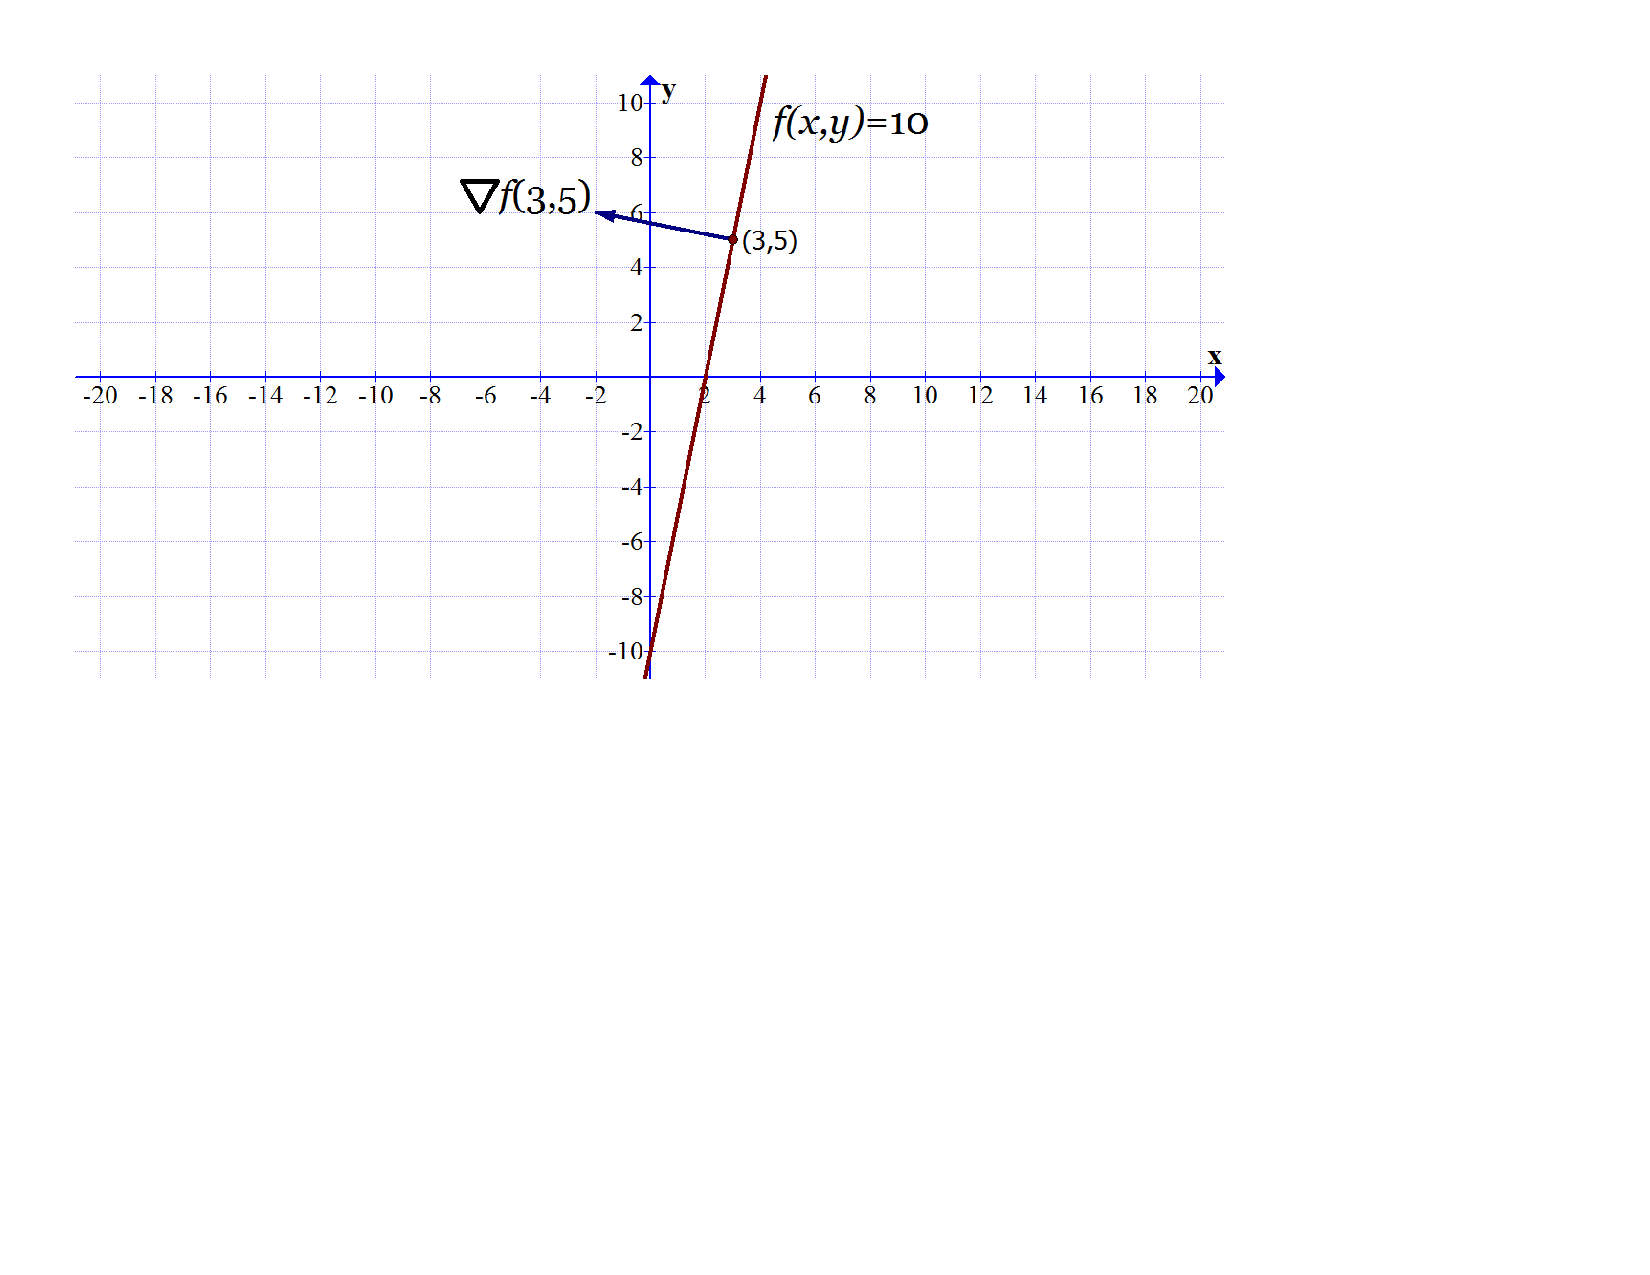
\includegraphics[scale=0.6]{normal.pdf}
\end{center}
}}} \fi

\item $f(x,y)=x^2+y^2$; $P\left(\frac{\sqrt{2}}{2},\frac{\sqrt{2}}{2}\right)$

\ifans{\fbox{\parbox{1\linewidth}{Point $P$ is on the level curve $f(x,y)=1$, i.e., $x^2+y^2=1$; $\nabla f \left(\frac{\sqrt{2}}{2},\frac{\sqrt{2}}{2}\right)=\left\langle \sqrt{2},\sqrt{2} \right\rangle$.
\begin{center}
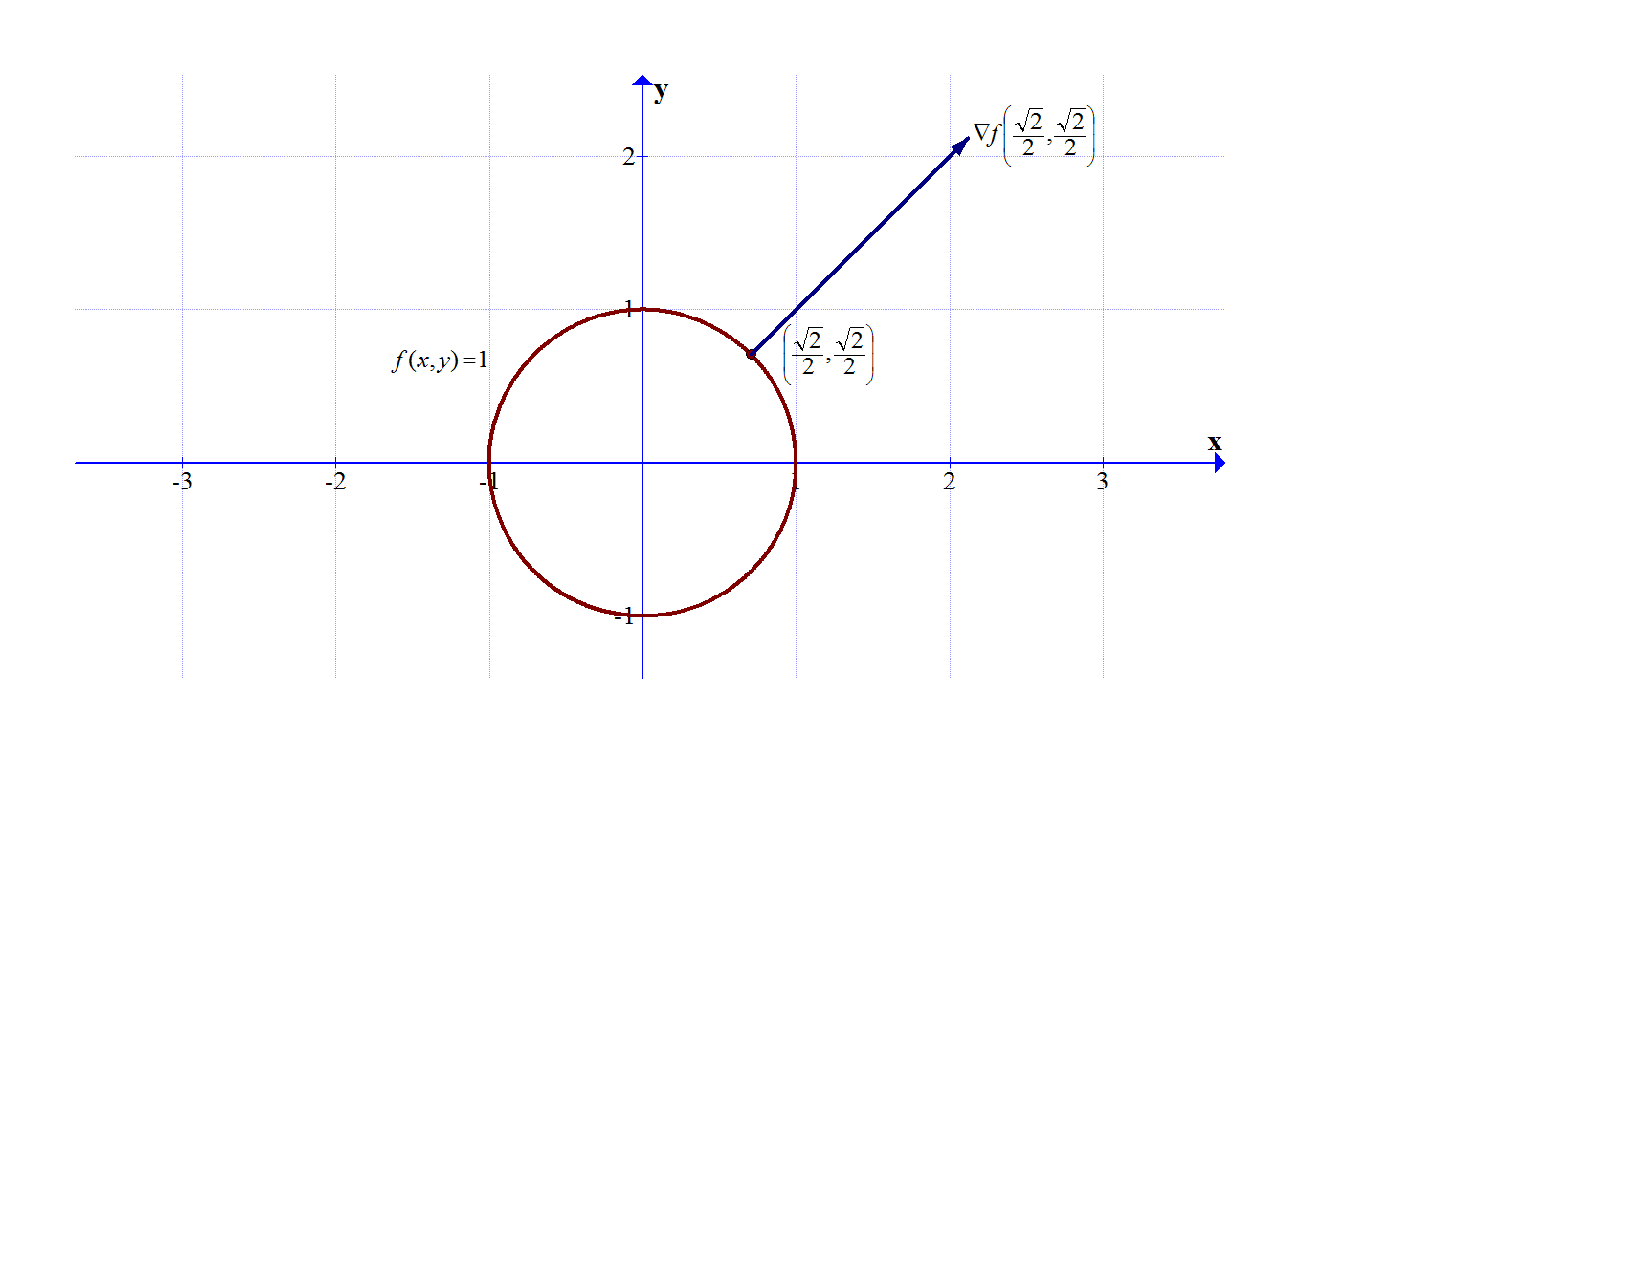
\includegraphics[scale=0.5]{normal2.pdf}
\end{center}
}}} \fi

\item The graph shown below depicts some level curves of an unspecified function $f(x,y)$.  

\begin{center}
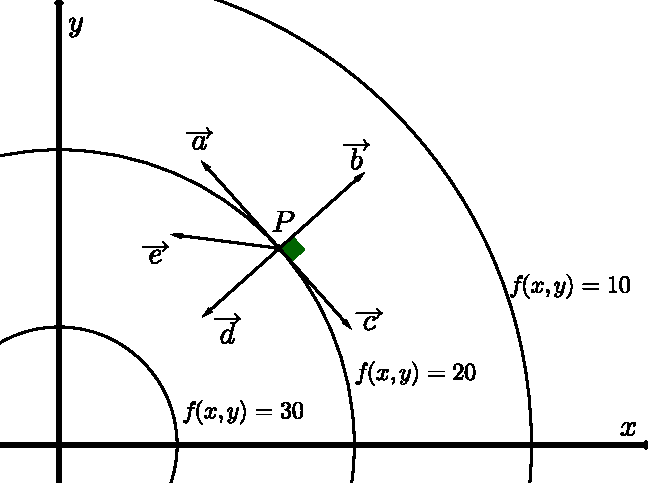
\includegraphics[scale=0.9]{gradient.pdf}
\end{center}

Which of the vectors is most likely to be $\nabla f$ at $P$?  Explain your reasoning.

\ifans{\fbox{\parbox{1\linewidth}{$\overrightarrow{d}$.  $\nabla f (P)$ should point in the direction of greatest increase and it should be normal to point $P$ on the level curve of $f(x,y)$.}}} \fi

\end{enumerate}

\end{document}